% TODO:
%   - Kijk na of titels in header overflowen
% ----------  
% Questions:
%   - XXX

% https://www.brainlatam.com/blog/wet-dry-active-and-passive-electrodes.-what-are-they-and-what-to-choose-413

% https://www.brainlatam.com/blog/a-brief-introduction-to-eeg-and-the-types-of-electrodes-75

% https://iopscience.iop.org/article/10.1088/1741-2552/abc902/pdf

% bci_review_book_chapter

% In a new chapter, reset the GLS to once again use full version in first occurence
\glsresetall

\chapter{Origins and acquisition of biomedical signals}
\label{ch:biomedical_signals}

% ---------------------------------------------- 
% INTRODUCTION
% ---------------------------------------------- 
\section{Introduction to this chapter}
\label{sec:biomedical_signals_introduction}
% NOTE: "Introduction" exists in each chapter and gives short intro to chapter + what can be expected in chapter

Whilst Chapter \ref{ch:bci} has provided an in-depth intuitive introduction to \glspl{bci}, some more technical aspects need addressing as well to provide a computer scientist with all of the required foundational knowledge for \gls{bci} research.
This chapter provides the required technical knowledge on the data that \gls{bci} systems use, brain signals.
Brain signals are only one of the many types of \gls{biosignal} present in the human body.
Whilst from a computer scientist's perspective brain signals may just be another type of input data to a classification model, having at least a basic understanding of this data is crucial in making good classification algorithms for \gls{bci} systems.
Even when using \gls{dl} approaches where no manual feature engineering has to be done and where basic models without much thought may have pleasing results, understanding the data will allow for the creation of better models.
This understanding of the data also helps in troubleshooting why some models may not have the desired results.

To provide this basic understanding, this chapter starts by briefly discussing \glspl{biosignal} in general.
It is discussed what \glspl{biosignal} are and where they originate from in the human body.
After this general discussion on \glspl{biosignal}, a focus is put on the different \glspl{biosignal} from the human brain, with brain signals measured using \gls{eeg} in particular.
This \gls{eeg} measuring technique and other measuring techniques are also discussed in greater detail.
Whilst it is addressed that \gls{eeg} has some fundamental shortcomings over other measuring modalities, it also has some attractive properties over these alternatives.
These attractive properties are listed and provide an argument as to why the remainder of this master thesis will focus on \gls{eeg} and \gls{mi} \gls{eeg} in particular.

% ---------------------------------------------- 
% ORIGINS
% ---------------------------------------------- 

\section{Biosignals in the human body}
\label{sec:biomedical_signals_biosignals_in_human}

In theory, a \glspl{biosignal} is nothing more than a measurement over time of a living
being.
In practice, these \glspl{biosignal} are closely related to physiological processes.
This makes it possible to monitor or detect those physiological processes using \glspl{biosignal}.
\Glspl{biosignal} can be produced by different energy forms, such as the electrical energy form when measuring \gls{eeg} in \gls{mv}.
Table \ref{tab:biomedical_signals_energy_forms} summarizes some of these energy forms and which type of \glspl{biosignal} they can produce.
Whilst living beings, including humans, produce many different types of \glspl{biosignal}, this master thesis will only consider time-varying electrical \glspl{biosignal}.
These types of \glspl{biosignal}, sometimes reffered to as \gls{elecbiosignal}, are the ones used as input data for \gls{bci} systems.
\Citet{biosignal_definition} discusses these and other types of \glspl{biosignal} in greater detail.

\begingroup
\setlength{\tabcolsep}{6pt} % Default value: 6pt
\renewcommand{\arraystretch}{2} % Default value: 1
\begin{table}[ht]
    \resizebox{\columnwidth}{!}{%
    \begin{tabular}{|l|p{5cm}|p{7cm}|}
        \hline
        \textbf{Energy form} & \textbf{Variable type}                 & \textbf{Biosignals}                                                                     \\ \hline
        Chemical             & Chemical activity and/or \newline concentration & Blood ions, O2, CO2, pH, hormonal \newline concentrations, and other chemistry                             \\ \hline
        Mechanical           & Position, force, torque or \newline pressure    & Muscle movement or cardiovascular pressures, muscle contractility, valve and other cardiac sounds \\ \hline
        Electrical           & Voltage or current                     & EEG, ECoG, ECG, EMG, EOG, ERG, EGG, GSR and EDA                                                                 \\ \hline
        Thermal             & Temperature                            & Body temperature and thermography                                                                    \\ \hline
        \end{tabular}%
        }
    \captionsetup{width=0.8\linewidth}
    \captionsetup{justification=centering}
    \caption{Some of the different energy forms in living beings and the most important measurable biosignals they produce. Data from \citet{biosignal_definition}.}
    \label{tab:biomedical_signals_energy_forms}
\end{table}
\endgroup

% - - - - - - - - - -
% how produced
% - - - - - - - - - -

\subsection{Origin of electricity inside the the human body}
\label{subsec:biomedical_signals_biosignals_electrical}

Electricity in the human body, better known as bioelectricity, can be seen as the generation or action of tiny electric currents and voltages in physiological processes.
As shown in Table \ref{tab:biomedical_signals_energy_forms}, the measurement of this bioelectricity is what enables the monitoring of \glspl{elecbiosignal}.
This is one of the reasons \glspl{biosignal} are closely related to physiological processes since it measures the bioelectricity used in some of these processes.
A complete understanding of how bioelectricity is made, maintained and transmitted in the human body isn't required for a computer scientist to contribute to the \gls{bci} field.
However, a superficial understanding of this process makes it easier to understand the limits of the accompanied \glspl{elecbiosignal}.
For this reason, the remainder of this section gives a simplified explanation of how bioelectricity is made, maintained and transmitted in the human brain.
This explanation is based on chapter 12 of the recently renewed book by \citet{bioelec_book}, an \gls{eeg} focused explanation of bioelectricity by \citet{eeg_bioelec_creation} and multiple YouTube videos by Neuroscientifically Challenged\footnote{\url{https://youtu.be/tIzF2tWy6KI}}\footnote{\url{https://youtu.be/W2hHt_PXe5o}}\footnote{\url{https://youtu.be/WhowH0kb7n0}}.

% | | | | | | | | | | | | |

\subsubsection{Resting membrane potential causes negatively charged neurons}
\label{subsubsec:biomedical_signals_biosignals_electrical_membrane_potential}

As was already addressed in Section \ref{subsec:bci_gaining_popularity_better_measuring}, the human brain has billions of neurons with \citet{neurons_book} stating that around $10^7$ parallel pyramidal neurons reside in only a single $cm^3$ of the brain cortex alone.
A neuron, also known as a nerve cell, is an electrically excitable cell.
Being an electrically excitable cell, a neuron has a resting membrane potential.
This resting membrane potential is around $-70$ \gls{milv} and expresses the difference in electrical charge between the inside and the outside of a neuron.
This negative difference is maintained by the sodium-potassium pump which is responsible for the hydrolysis of ATP to ADP.
During this hydrolysis process the sodium-potassium pump releases three positively charged sodium ions ($Na^+$) whilst only taking in two positively charged potassium ions ($Ka^+$), this difference causes the membrane potential to remain negative.

% | | | | | | | | | | | | |

\subsubsection{Action potential allows for neuron communication}
\label{subsubsec:biomedical_signals_biosignals_electrical_action_potential}

Whilst the sodium-potassium pump inside the neuron explains why there is a negative resting membrane potential of around $-70$ \gls{milv}, it doesn't explain the variable volt measurements of \gls{eeg}.
The change in membrane potential occurs when the neuron gets excited.
The most common way a cell gets excited is through the process known as an action potential.
An action potential forms the basis for electrical signalling within neurons, enabling some form of communication between them.
To do this communication, neurotransmitters released by another neuron bind to receptors on the dendrites of the receiving neuron which has a depolarization effect.

This depolarization causes the neuron to become less polarized, resulting in its membrane potential moving close to zero.
When sufficient depolarization occurs, the action potential process could start.
This process is visualised in Figure \ref{fig:biomedical_signals_action_potential}.
For the action potential process to start, the depolarization should be of such a magnitude that the neuron reaches its threshold membrane potential, which is around $-55$ \gls{milv}.
This is achieved through the repeated binding of neurotransmitters to the receptors.
The annotation for "failed initiations" in Figure \ref{fig:biomedical_signals_action_potential} denotes the common situations when the threshold membrane potential is not reached.

When the threshold is reached, a large number of sodium channels open, allowing many positive sodium ions ($Na^+$) into the neuron, causing the membrane potential to rise quickly.
This depolarization is what creates the electrical signal known as the action potential that travels down the neuron to eventually release neurotransmitters itself.
Eventually, a peak is reached, after which the sodium channels close, not allowing any further sodium ions ($Na^+$) to enter the neuron.
To return to its resting membrane potential, the neuron opens its potassium channels to release many potassium ions ($Ka^+$).
This is known as the falling phase where the neuron repolarizes.
However, the release of positive potassium ions ($Ka^+$) happens so quickly that the membrane potential falls below the resting membrane potential.
The neuron is now hyperpolarized, denoted as undershoot in Figure \ref{fig:biomedical_signals_action_potential}.
During this hyperpolarized state, also known as the refractory period, failed initiations occur more often as it is very difficult to fire the neuron again.
Eventually, the resting membrane potential is reached again and the neuron functions like before.


\begin{figure}[ht]
    \centering
    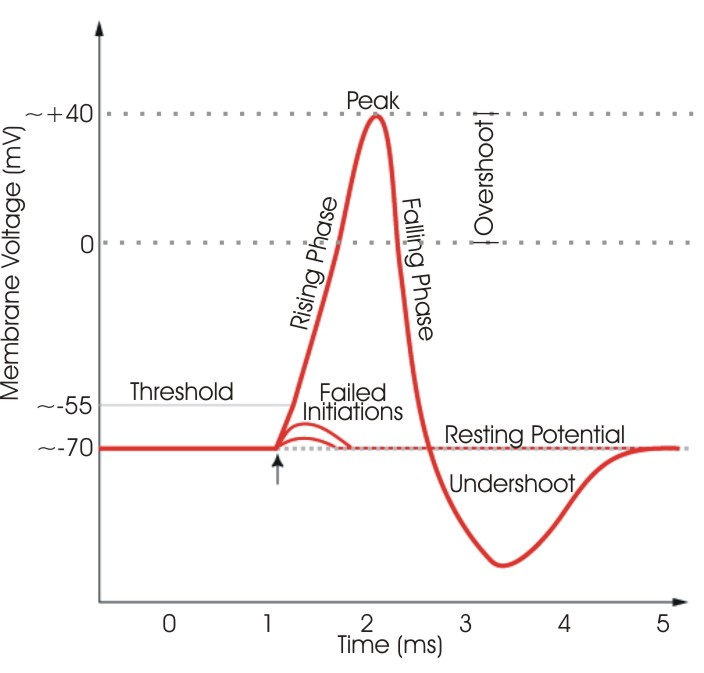
\includegraphics[width=0.7\linewidth]{../images/biosignals/action_potential.jpg}
    \captionsetup{width=0.7\linewidth}
    \captionsetup{justification=centering}
    \caption{Chart of the membrane potential during the action potential process in a neuron. Figure from Synaptidude, GFDL 1.2, via Wikimedia Commons.} 
    \label{fig:biomedical_signals_action_potential}
\end{figure}



% | | | | | | | | | | | | |

\subsubsection{EEG measures postsynaptic potentials}
\label{subsubsec:biomedical_signals_biosignals_electrical_postsynaptic_potential}

Whilst the action potential explains how most changes in membrane potential of an individual neuron occur, it is highly unlikely to be measured by \gls{eeg} and other measuring modalities.
This follows from the fact that, as discussed earlier, many billion neurons make up the brain making it impossible to monitor a singular neuron.
Since action potentials are such rapid current flows, it is highly unlikely enough neighbouring neurons will have an action potential at the same time resulting in a measurable signal.
However, whilst it was discussed how neurotransmitters can cause depolarization which can initialize action potentials, these neurotransmitters can also influence the membrane potential in the opposite direction by causing further polarization.
The release of these neurotransmitters and the binding to the receiving neuron also causes currents known as postsynaptic potentials.
Whilst these are not action potentials, they are essentially what causes an action potential to take place and the action potential can also cause the release of neurotransmitters.
These postsynaptic potentials are present for a longer period than action potentials.
Thus, it is more likely for many neighbouring neurons to have active postsynaptic potentials simultaneously.
The summation of these postsynaptic potential currents from many millions of neurons is what is detected by \gls{eeg}.
However, neurons experiencing action potential at that same time are among many other things sources of noise in this summation of these currents.
\Citet{what_eeg_is_and_measures} explain in greater detail what exactly is measured with \gls{eeg}.



% | | | | | | | | | | | | |

\subsubsection{Biosignals originating from bioelectricity in the human body}
\label{subsubsec:biomedical_signals_biosignals_electrical_biosignals}

Both voltage and current can be measured from bioelectricity, providing many different \glspl{biosignal}.
The measurement of voltage originating from the brain, measured in a non-invasive manner with electrodes on the scalp is known as \gls{eeg}.
Likewise, \gls{ecg} revolves around the non-invasive measurement of voltage originating from the heart.
\Gls{eog} and \gls{erg} are techniques used for measuring bioelectricity that originates from the eyes.
Table \ref{tab:biomedical_signals_energy_forms} provides the most important \glspl{biosignal} related to the measurement of bioelectricity.
The most important \gls{elecbiosignal} in BCI research are \gls{eeg} and the invasive alternative \gls{ecog}.


% - - - - - - - - - -
% Other energy forms
% - - - - - - - - - -

\subsection{Other energy forms and their related biosignals}
\label{subsec:biomedical_signals_biosignals_others}

Section \ref{subsec:biomedical_signals_biosignals_electrical} illustrated that bioelectricity is omnipresent in the human body. 
The human nervous system relies on bioelectricity to quickly carry information from the human body to the brain and the other way around.
The process of muscle contraction is started when the discussed action potentials release neurotransmitters from motor neurons to muscle fibres.
As discussed by \citet{bioelectricity_cancer}, bioelectricity can even be \textit{hijacked} as a way of novel medicine and treatment, i.e. for cancer treatment.

However, bioelectricity is only one energy form present in the human body.
As shown in Table \ref{tab:biomedical_signals_energy_forms}, other energy forms provide many other types of \glspl{biosignal}.
Whilst these are of great importance in many fields, \gls{bci} research is mostly interested in brain activity and thus the \glspl{elecbiosignal} \gls{eeg} and \gls{ecog}.
However, as discussed in Section \ref{subsubsec:bci_common_use_cases_improving_existing_system_smart_home}, hybrid systems are being explored which may combine these \glspl{elecbiosignal} with \glspl{biosignal} from other energy forms.
These types of hybrid systems and the other types of \glspl{biosignal} they use fall outside the scope of this master thesis.

% ---------------------------------------------- 
% MEASURING BRAIN SIGNALS
% ---------------------------------------------- 

\section{Measuring biosignals from the brain}
\label{sec:biomedical_signals_measuring_brain}

Neuroimaging is a discipline focused on capturing the anatomy and function of the \gls{cns}, which includes the brain \citep{neuroimaging}.
As such, the modalities for measuring biosignals in the brain are mostly a subcollection of neuroimaging techniques.
Many different types of these modalities exist, both invasive and non-invasive.
There is no singular best measuring modality and often a trade-off has to be made between affordability, the \gls{snr}, the ease-of-use and the risks involved.
Section \ref{subsec:biomedical_signals_measuring_brain_modalities} will discuss these modalities in further detail.
The remainder of this master thesis then focuses on the \gls{eeg} modality as it remains one of the most attractive modalities for \gls{bci} research.



% - - - - - - - - - -
% Measuring modalities
% - - - - - - - - - -

\subsection{Common measuring modalities in BCI systems}
\label{subsec:biomedical_signals_measuring_brain_modalities}

Research by \citet{human_eeg_discovery} is the first in describing the measurement of brain waves from the human brain in a non-invasive manner.
Because of this, the German neuroscientist and psychiatrist Hans Berger is often seen as the inventor of \gls{eeg}.
Whilst he was one of the first to use the term \textit{elektrenkephalogramm}, it was Richard Caton who first described the findings of bioelectricity in brains in general.
He found this phenomenon in animal brains as early as 1875 \citep{first_eeg}.
Since then, the neuroimaging field has been looking for new ways to capture these electrical signals coming from the brain and monitor the anatomy and function of the \gls{cns} in general.
This has caused the introduction of many different measuring modalities, each with its strengths and weaknesses.
However, many of these modalities require bulky equipment which makes them non-portable and thus non-attractive for use in general \gls{bci} systems \citep{modalities_review1}.

Table \ref{tab:biomedical_signals_modalities} provides an overview of the most common measuring modalities considered for use in \gls{bci} applications together with some of their properties.
Many more modalities exist but these are currently not portable enough or have not yet been proven useful for use in \glspl{bci} \citep{modalities_review1, modalities_review2}.
Modalities based on the presence of \glspl{elecbiosignal} in the human brain seem most probable to be used in \gls{bci} systems for the foreseeable future \citep{modalities_review2}.
This includes \gls{eeg}, \gls{ecog}, intravascular electrodes and implemented electrodes among other modalities.
However, there is also a growing interest in using modalities working with non-electrical signals for \gls{bci} applications.
Whilst these are still limited due to poor portability and affordability, they have promising aspects for future research.
This section focuses on some of the most important modalities for \gls{bci} research.
The works by \citet{modalities_review1} and \citet{modalities_review2} cover some more modalities in greater detail.


\begingroup
\setlength{\tabcolsep}{6pt} % Default value: 6pt
\renewcommand{\arraystretch}{2} % Default value: 1
\begin{table}[ht]
    \resizebox{\columnwidth}{!}{%
    \begin{tabular}{|l|l|l|l|l|l|l|l|l|}
        \hline
        Modality                   & Invasive & Risks  & Temporal resolution & Spatial resolution & Affordability & Ease-of-installation & Ease-of-use & Comfort \\ \hline
        EEG                        & No       & Low    & 50ms                & 10mm               & €             & Good                 & Good        & Medium  \\ \hline
        ECoG                       & Yes      & High   & 5ms                 & 1mm                & €€-€€€        & Poor                 & Good        & Good    \\ \hline
        fNIRS                      & No       & Low    & 1000ms              & 10mm               & €-€€€        & Good                 & Good        & Medium  \\ \hline
        Implemented microelectrode & Yes      & High   & 3ms                 & 0.05mm - 0.5mm     & €€€           & Poor                 & Good        & Good    \\ \hline
        Intravescular electrode    & Yes      & Medium & 5ms                 & 2.4mm              & €€-€€€        & Poor                 & Good        & Good    \\ \hline
        fTCD                       & No       & Low    & 1000ms - 5000ms     & 10mm - 30mm        & €             & Medium               & Medium      & Poor    \\ \hline
        MEG*                       & No       & Low    & 1ms - 5ms           & 1mm                & €€€+          & Good                 & Poor        & Poor    \\ \hline
        \end{tabular}%
        }
    \captionsetup{width=0.9\linewidth}
    \captionsetup{justification=centering}
    \caption{Overview of the most common neuroimaging modalities for use in BCI systems. *: Currently not available in a portable manner. Data based on \\\citet{modalities_review1} and \citet{modalities_review2}.}
    \label{tab:biomedical_signals_modalities}
\end{table}
\endgroup


% | | | | | | | | | | | | |

\subsubsection{Electroencephalography (EEG)}
\label{subsubsec:biomedical_signals_measuring_brain_modalities_eeg}

\Glsfirst{eeg} is a non-invasive technique used to measure the electrical activity of the brain, often expressed in \gls{mv} over time.
Electrodes are most commonly placed on the scalp with as main goal to detect the activity of neurons in the cerebral cortex.
The cerebral cortex, better known as grey matter, is the outmost layer of the brain, closest to the electrodes placed on the scalp.
Whilst more inner layers of the brain also produce information-rich \gls{elecbiosignal}, these signals do not reach the scalp in a clear detectable manner for \gls{eeg} to pick up.
As discussed in Section \ref{subsec:biomedical_signals_biosignals_electrical}, \gls{eeg} is not capable of measuring the individual activity of neurons in the cerebral cortex but rather the activity of large groups of neurons that are active at the same time.
Postsynaptic potentials contribute most to these measurements as action potentials are too short in duration.
The location at which electrodes are placed on the scalp often follows specific standards which are further explained in Section \ref{subsec:biomedical_signals_working_with_eeg_standards}.
These electrodes can be divided based on whether they are wet or dry, active or passive and whether they are wired or wireless.
The difference between these types has already been covered in Section \ref{subsec:bci_gaining_popularity_better_measuring}.

The output of these electrodes is processed through a differential amplifier which takes two electrical inputs and displays the output as the difference between these inputs.
This means that an \gls{eeg} measurement displayed from one electrode is not absolute but rather the relative difference between that electrode and another.
The selection of the other electrode for passing through the differential amplifier can differ per device through what is known as the montage of the \gls{eeg} device.
The most common montages are common reference, average reference and bipolar.
The common reference montage uses a predefined electrode as a reference electrode and compares each electrical signal from an electrode with it.
Most commonly this reference electrode is placed on the ear as this is least influenced by brain activity.
The average reference montage compares each electrical signal from an electrode with the averaged electrical signal from all electrodes.
The bipolar montage follows a certain scheme of comparing two always differing electrodes with each other.
Most often this is done in a sequence from the front of the scalp to the back of the scalp.
All of these montages are summarized in Figure \ref{fig:biomedical_signals_eeg_montages}.
The output of the differential amplifier is what is known as the \gls{eeg} measurement.

\begin{figure}[ht]
    \centering
    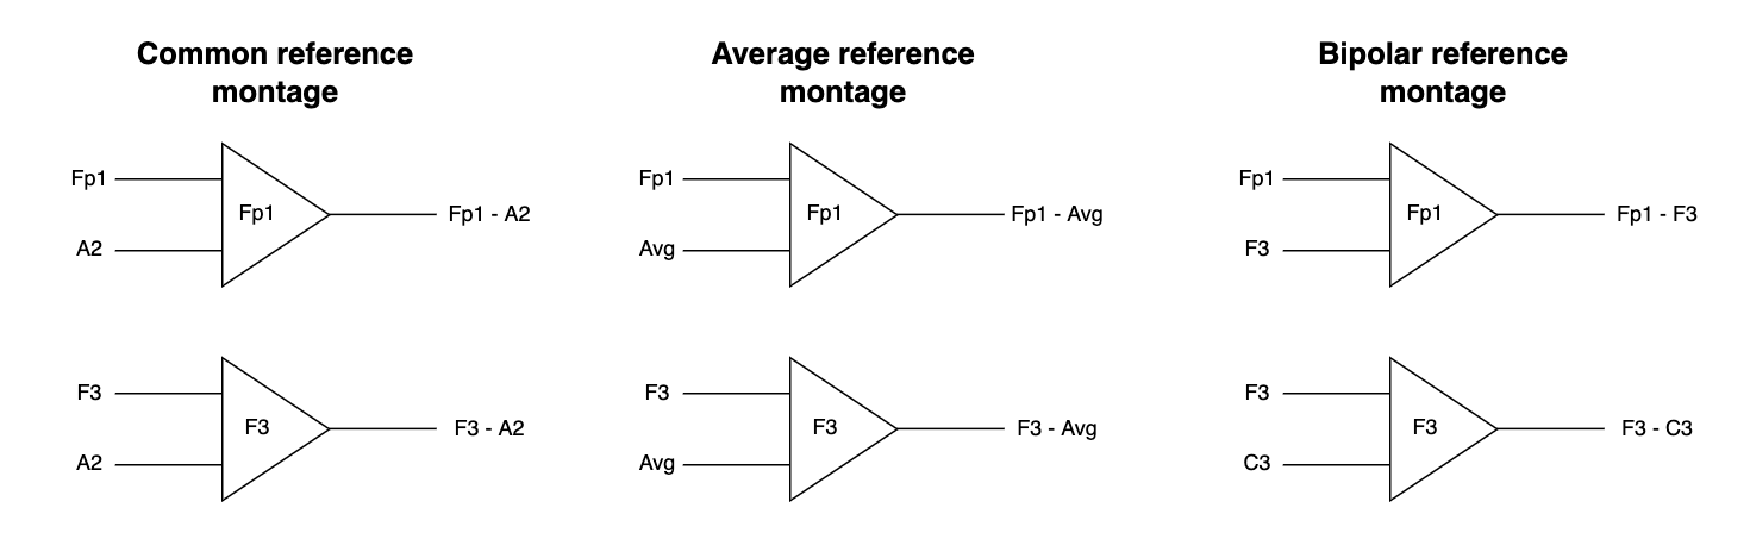
\includegraphics[width=\linewidth]{../images/eeg/montages.pdf}
    \captionsetup{width=0.8\linewidth}
    \captionsetup{justification=centering}
    \caption{Illustration of the three most common montages for the differential amplifier in EEG. The annotations are the electrode names used in the international 10-20 system.} 
    \label{fig:biomedical_signals_eeg_montages}
\end{figure}

\Gls{eeg} is one of the most popular neuroimaging modalities and also the most common modality in \gls{bci} research \citep{modalities_review1, modalities_review2, bci_review_arnau}.
This success is due to the good temporal resolution, its non-invasive nature and the relatively low cost of \gls{eeg} hardware, further discussed in Section \ref{subsec:biomedical_signals_measuring_brain_equipment}.
Many different types of headsets and caps exist which hold the electrodes in place and with minimal modification, these headsets are easy to install and use, which is also an attractive property of \gls{eeg}.

However, some of the headsets for dry electrodes, such as the Ultracortex Mark IV discussed in Section \ref{subsec:bci_opportunities_obstacles_motivating_examples}, can be unpleasant to wear over prolonged sessions.
Other disadvantages include the poor spatial resolution as discussed in Section \ref{subsec:bci_gaining_popularity_better_measuring}.
This poor spatial resolution combined with multiple fluids and structures blocking the electrical signals coming from the brain means that the data collected from \gls{eeg} is relatively low in quality, both from a \gls{snr} perspective and a source localisation perspective.
Since \gls{eeg} measurements are limited to the activity of neurons in the grey matter, not all brain activity can be measured by \gls{eeg} either.
Section \ref{subsec:biomedical_signals_biosignals_electrical} and \citet{what_eeg_is_and_measures} explain in greater detail what \gls{eeg} effectively measures.
Some studies have also shown that extensive \gls{eeg} use can cause temporary hair loss and the electrolytic gel could also cause allergic effects for the user \citep{eeg_hair_loss, dry_electrode_status}.




% | | | | | | | | | | | | |

\subsubsection{Electrocorticography (ECoG) and other invasive methods}
\label{subsubsec:biomedical_signals_measuring_brain_modalities_ecog}

With most shortcomings of \gls{eeg} being related to the non-invasive nature of the modality, invasive variants of \gls{eeg} have been studied extensively as well.
One such invasive modality to measure the \gls{elecbiosignal} of the brain is \glsfirst{ecog}.
When using \gls{ecog}, electrodes are placed directly on the cerebral cortex, the outer layer of the brain.
\Gls{ecog} was first explored in the 1950s to determine the exact origin of epileptic seizures so that this part of the brain could be surgically removed \citep{ecog_origin}.
The procedure used involved opening a portion of the skull, placing the electrodes on the exposed area of the cerebral cortex, waiting for a seizure to occur such that \gls{ecog} can be used to determine the exact location, removing that part of the brain, removing the electrodes and closing the skull again.
This was done in this manner as the electrodes are physically closer to the brain, improving the spatial resolution and \gls{snr} significantly when compared to \gls{eeg}.
To this day, \gls{ecog} is still used in certain brain surgeries and this type of use of \gls{ecog} is called \textit{intraoperative} \gls{ecog}.

However, this superior spatial resolution, far better \gls{snr} and the relatively fixed electrode positioning combined with a system that is invisible to the human eye has made it an attractive variant of \gls{eeg} for post-surgery measurements as well.
This is known as \textit{extraoperative} \gls{ecog}.
Many successful steps have been made to lower the risk and costs associated with the invasive nature of \gls{ecog}.
When only interested in \textit{extraoperative} \gls{ecog}, a craniotomy, also known as an open skull surgery, is not needed anymore.
Instead, tiny holes can be made in the skull to implement the electrodes in that way.
The size and associated surgical risks of those holes have been shrinking.

The Neuralink company discussed in Section \ref{subsec:bci_gaining_popularity_better_measuring} is responsible for the most recent advancements in this area, with the implantation of hair-sized electrodes being capable using only a robot and minimal anaesthesia.
At this stage, it is unclear whether their system will be considered \textit{extraoperative} \gls{ecog} or a different type of invasive measuring modality.
Since these electrodes are so tiny, many thousands could be used for measuring the brain signals, compared to \gls{eeg} where a system with 21 or 64 electrodes is most common.
Whilst for \gls{eeg} having more than 1024 electrodes is almost impossible due to the physically limited space on the scalp, invasive techniques are aiming to allow for thousands of electrodes in only a small region of the brain.
Whether this increase in electrodes will be useful has yet to be determined, as for \gls{eeg} it is known that adding more electrodes does not improve the measured information past a certain point \citep{dropping_curve_eeg_lectrodes, more_electrodes_not_better}.
However, many of these procedures still need significant medical trials before widespread use will be possible and as such, \gls{ecog} and other invasive methods such as intravascular electrodes (minimally invasive) and implemented microelectrodes (best spatial resolution) are yet to see widespread \gls{bci} adoption outside medical applications.
These latter invasive methods are covered in more detail by \citet{modalities_review1}.
There are also some ethical questions surrounding the use of invasive \gls{bci}, as discussed in Section \ref{subsec:bci_ethical_e_waste}.


% | | | | | | | | | | | | |

\subsubsection{Other modalities which do not rely on bioelectricity}
\label{subsubsec:biomedical_signals_measuring_brain_modalities_others}

As discussed in Section \ref{sec:biomedical_signals_biosignals_in_human}, there are multiple energy forms that produce \glspl{biosignal}.
Measuring electrical signals from the brain is by far the most common in \gls{bci} research as these \glspl{elecbiosignal} carry much information surrounding brain activity whilst also being relatively easy to measure.
The discussed \gls{eeg}, \gls{ecog}, intravascular electrodes and implemented electrodes all measure \glspl{elecbiosignal}.
Besides measuring \glspl{biosignal} which are being emitted by the human body all the time, it is also possible to expose the human body to an external energy form and measure the reaction of the human body.
These types of modalities are common for medical imaging in hospitals.
The popular X-ray, \gls{ct}, \gls{pet} and \gls{spect} imaging modalities all rely on different forms of ionising radioactive exposure to the human body.
Non-ionising methods are also common, such as the \gls{mri} modality which relies on exposing the body to strong electrical fields.

Some of these medical imaging modalities have seen use in highly medical \gls{bci} applications, but they require expensive and non-portable equipment, which makes them unsuited for use in general use \gls{bci} systems and conflicting with Wolpaw's definition of a perfect \gls{bci} given in Section \ref{sec:bci_introduction} \citep{modalities_review1,modalities_review2}.
One very promising medical imaging technology for measuring brain activity is \gls{meg}.
Intuitively, \gls{meg} could be seen as an alternative to \gls{eeg} that measures the magnetic activity associated with brain activity rather than the electrical activity.
\Gls{meg} distinguishes itself from other modalities by offering excellent temporal and spatial resolution whilst being non-invasive and without any mentionable risk.
These properties make \gls{meg} an incredibly attractive modality for use in \gls{bci} research.
However, the device required to perform a \gls{meg} scan costs millions, is non-portable and requires high maintenance in its current form.
This makes it unsuited for general \gls{bci} usage and only highly medical and temporary \gls{bci} applications have been made with it \citep{modalities_review2}.
If \gls{meg} would ever become portable and affordable it is bound to revolutionise the \gls{bci} field.
\Citet{meg_explained} explains the \gls{meg} modality in greater detail.

A technique that has seen such a decrease in price and increase in portability is \gls{fnirs}.
As shown by \citet{fnirs_cheap}, a comfortable and portable \gls{fnirs} headset can be made for only a few hundred euros, compared to previously available solutions which cost thousands and are less portable and comfortable.
\Gls{fnirs} thanks its name due to the use of a light source that operates near the infrared wavelength for detecting changes in haemoglobin species present in the brain.
\Gls{fnirs} does not expose the body to ionising radiation and is proven to be a safe modality for repeated use \citep{fnirs_explained}.
Whilst the poor temporal resolution of \gls{fnirs} limits it usability for online \gls{bci} systems where a fast response time is desired, it has been used in combination with \gls{eeg} to form a successful hybrid-\gls{bci} \citep{modalities_review1, eeg_fnirs_drone}.
\Citet{fnirs_explained} explains the \gls{fnirs} modality in more detail.


% - - - - - - - - - -
% Why EEG
% - - - - - - - - - -

\subsection{The attractiveness of non-invasive EEG for BCIs}
\label{subsec:biomedical_signals_measuring_brain_why_eeg}

It is clear from table \ref{tab:biomedical_signals_modalities} that invasive modalities for measuring \glspl{elecbiosignal} from the brain generaly have excellent spatial and temporal resolution.
Adding to this, the invasive device is always present and ready to be used once implanted and if the implantation procedure has no side effects, the user comfort and easy-to-use factor of these approaches should also be among the best.
With electrodes being physically closer to the brain, the \gls{snr} and other data quality metrics are also often superior compared to non-invasive alternatives.
All of these properties point towards invasive solutions being superior to non-invasive alternatives for \glspl{bci} applications.

However, there are also some major drawbacks to invasive solutions.
As discussed in Section \ref{subsec:bci_ethical_e_waste}, ethical questions on what happens to an invasive \gls{bci} once it eventually stops working or stops receiving support are challenging to answer.
Other ethical questions present for \glspl{bci} in general, such as data privacy discussed in \ref{subsec:bci_ethical_data_mining}, are even more challenging for invasive approaches, as they can't simply be removed when the user wants to ensure the device is not active.
Besides these ethical issues, there are also still significant medical risks and high costs associated with these invasive solutions.
Whilst an automated implantation procedure is likely to reduce both costs and risks, as already demonstrated by \citet{neuralink_whitepaper}, there is no widespread availability possible yet.

Given the risks, high costs and limited availability still associated with invasive approaches, this master thesis and most research active in the field still focus on non-invasive solutions.
From these available modalities, \gls{eeg} is the oldest but also the most studied.
It's been proven capable of making multiple \gls{bci} applications possible as discussed throughout Chapter \ref{ch:bci}.
The good temporal resolution, affordability and \gls{ux} for headset installation, use and comfort make \gls{eeg} attractive over other non-invasive modalities.
The limited spatial resolution and poorer \gls{snr} are downsides but can be taken into account when developing a \gls{bci} system.
This is what makes \gls{eeg} attractive in current \gls{bci} research and why it remains so common and the modality of focus for this master thesis.

The choice between invasive and non-invasive solutions is an open discussion in the \gls{bci} field as \citet{bci_invasive_or_not1} and \citet{bci_invasive_or_not2} discuss in greater detail.
Once invasive systems become safer and more affordable, only time will tell how the ethical challenges will influence a potential future dominance of invasive solutions.
Given non-invasive solutions such as \gls{meg} have proven to be far superior to \gls{eeg} and even some invasive alternatives, further evolution in affordability and portability of these modalities are likely to leave the debate between invasive and non-invasive solutions ongoing for a long time.

% - - - - - - - - - -
% available equipment
% - - - - - - - - - -

\subsection{Available EEG measuring equipment}
\label{subsec:biomedical_signals_measuring_brain_equipment}

With \gls{eeg} being one of the oldest brain signal measuring modalities, many devices for the acquisition of \gls{eeg} have been introduced.
Some consumer-grade \gls{eeg} devices, such as the Neurosky Mindwave Mobile 2, only use a singular electrode for capturing brain signals whilst some medical-grade devices, such as the g. Pangolin High density EEG, boast up to 1024 electrodes \citep{bci_cheap_viability5}.
Likewise, most consumer-grade \gls{eeg} devices offer a sensible 256 \gls{hz} to 512\gls{hz} sampling frequency whilst some medical devices, such as the ANT Neuro eego my lab 256, support up to a 16000\gls{hz} sampling frequency and more.
As discussed in Section \ref{subsec:biomedical_signals_measuring_brain_modalities} and \ref{subsec:bci_gaining_popularity_better_measuring}, there are also various types of electrodes that can be used.
This means that hardware capable of measuring \gls{eeg} can start anywhere from a couple of hundred euros to multiple tens or even hundreds of thousands of euros.

Many comparisons between different types of measuring equipment, often with greatly differing costs, have already been made \citep{bci_cheap_viability1, bci_cheap_viability2, bci_cheap_viability3, bci_cheap_viability4, bci_cheap_viability5, low_cost_eeg_devices, muse_comparison}.
Table \ref{tab:biomedical_signals_eeg_equipment} shows some of the available \gls{eeg} measuring equipment and their specifications.
Comparing all of these devices falls outside the scope of this master thesis but the remainder of this section will highlight the meaning of the provided specifications.


\begingroup
\setlength{\tabcolsep}{6pt} % Default value: 6pt
\renewcommand{\arraystretch}{2} % Default value: 1
\begin{sidewaystable}
    \resizebox{\columnwidth}{!}{%
    \begin{tabular}{|l|l|l|l|l|l|l|l|l|l|}
        \hline
        \textbf{Company}          & \textbf{Product} & \textbf{Price estimate} & \textbf{Electrode count} & \textbf{Electrode type} & \textbf{Sampling frequency} & \textbf{Headset aesthetics} & \textbf{Customizability} & \textbf{Wireless} & \textbf{Python support} \\ \hline
        NeuroSky                  & Mindwave         & €150                    & 1                        & Dry                     & 512Hz                       & Good                        & Poor                     & Yes               & Minimal                 \\ \hline
        InteraXon                 & Muse 2           & €270                    & 4                        & Dry                     & 256Hz                       & Good                        & Poor                     & Yes               & Good                    \\ \hline
        OpenBCI                   & Ganglion         & €800                    & 4                        & Variable (active dry)   & 200Hz                       & Variable (poor)             & Good                     & Yes               & Good                    \\ \hline
        OpenBCI                   & Cyton            & €1500                   & 8                        & Variable (active dry)   & 250Hz                       & Variable (poor)             & Good                     & Yes               & Good                    \\ \hline
        Emotiv                    & Epoc Flex        & €2000                   & 32                       & Variable (passive wet)  & 128Hz                       & Decent                      & Decent                   & Yes               & Good                    \\ \hline
        OpenBCI                   & Cyton + Daisy    & €2500                   & 16                       & Variable (active dry)   & 125Hz-250Hz                 & Variable (poor)             & Good                     & Yes               & Good                    \\ \hline
        Neuroelectrics            & Enobio 20        & €10000+                 & 20                       & Wet                     & 500 Hz                      & Decent                      & Decent                   & Yes               & Good                    \\ \hline
        Advanced brain monitoring & B-Alert X24      & €10000+                 & 20                       & Wet                     & 256Hz                       & Poor                        & Decent                   & Yes               & Poor                    \\ \hline
        Wearable Sensing          & DSI 24           & €20000                  & 24                       & Dry                     & 600Hz                       & Poor                        & Poor                     & Yes               & Minimal                 \\ \hline
        ANT Neuro                 & eego mylab 256   & €25000+                 & 256                      & Wet                     & 16000Hz                     & Decent                      & Poor                     & No                & Minimal                 \\ \hline
        \end{tabular}%
        }
    \captionsetup{width=0.9\linewidth}
    \captionsetup{justification=centering}
    \caption{Some of the available EEG measuring equipment with their most important specifications. Some equipment consists of multiple configurable components, these are annotated as "variable" with the default option provided in brackets. Prices are estimates based on buying a minimal total configuration of the product. Data was gathered from the original manufacturer's website and community blogs. More information on the provided properties is given in Section \ref{subsec:biomedical_signals_measuring_brain_equipment}.}
    \label{tab:biomedical_signals_eeg_equipment}
\end{sidewaystable}
\endgroup


% | | | | | | | | | | | | |

\subsubsection{Pricing of EEG equipment}
\label{subsubsec:biomedical_signals_measuring_brain_equipment_pricing}

% Research showing OpenBCI Cyton to be comparable to 25x more expensive bioamplifier

Prices of \gls{eeg} measuring equipment vary a lot.
Cheap consumer-grade systems like the InteraXon Muse 2 can be bought for under €300.
These types of systems are often considered novelty items, as their limited electrode counts combined with poor \gls{snr} is believed to limit their capabilities as part of a \gls{bci} system.
However, the InteraXon Muse 2 has been proven to have good support in Python libraries and other programming languages.
This has caused many individuals and researchers to try the headset, which has resulted in a broad range of commercial \gls{bci} applications, proving both its educational and overall usefulness is greater than the specifications would suggest \citep{muse_comparison}.
Research-grade equipment like the OpenBCI Cyton, OpenBCI Cyton + Daisy and Emotiv Epoc Flex can be bought for around €2000, which includes the main board, electrodes and a headset or cap for holding those electrodes.
Medical-grade \gls{eeg} hardware has to have specific licenses and approvals which increases the costs significantly.
Since these medical-grade devices are bought for a specific medical application and thus are often bundled with software, exact prices are rarely stated online.
However, known prices for medical \gls{eeg} equipment are well above €10000, with more than double that not being uncommon when paired with capable software.


% | | | | | | | | | | | | |

\subsubsection{Electrode type and count of EEG equipment}
\label{subsubsec:biomedical_signals_measuring_brain_equipment_electrodes}

Cheap consumer-grade hardware often focuses on a pleasant \gls{ux} rather than raw data quality.
Because of this, these cheaper systems often make use of only a small number of dry electrodes in an all-in-one package.
Research-grade hardware is often more flexible in this regard, with main boards that can work with both wet and dry electrodes through universal connectors that allow for many different types of electrodes to be connected.
Most of these research-grade headsets even support other types of sensors, such as \gls{emg} electrodes, to be connected as well. 
The electrode count of these research-grade devices is often around 20, as it aims to be compatible with the international 10-20 system discussed in Section \ref{subsec:biomedical_signals_working_with_eeg_standards}.
Medical grade systems often aim for the highest data quality possible, using expensive golden wet electrodes.
Whilst most of these systems offer interchangeable electrodes as well, they often use proprietary connectors which limits the choice of electrodes significantly.
Electrode counts of some expensive medical-grade systems are also multitudes higher than those of other hardware, with 256 electrodes not being uncommon.
However, this increased electrode count does not guarantee an increase in information captured, as already touched upon in Section \ref{subsec:bci_gaining_popularity_better_measuring}.
Experiments by \citet{ideal_eeg_electrode_count_place} revealed that 32 well-placed electrodes could be sufficient for most \gls{eeg} applications.

% | | | | | | | | | | | | |

\subsubsection{Sampling frequency of EEG equipment}
\label{subsubsec:biomedical_signals_measuring_brain_equipment_sampling_frequency}

% CYTON + DAISY
% The CytonDaisy Board samples data at 125 Hz on each of its 16 channels. However, if you select the "save data to microSD card" option in the OpenBCI GUI, you can take advantage of the 250 Hz sampling rate.

The sampling frequency of \gls{eeg} equipment is often expressed in \glsfirst{hz} and corresponds to the number of samples taken from every electrode per second.
When taking into account the Nyquist sampling theorem, the sampling frequency should be at least twice the highest frequency contained in the signal that is being measured \citep{nyquist_theory}.
Considering the highest frequency of the five widely recognized brain waves discussed in Section \ref{subsec:biomedical_signals_working_with_eeg_brain_waves} is 100\gls{hz} for the gamma waves, a minimal sampling frequency of 200\gls{hz} is common for \gls{eeg} equipment.
However, based on the applications, the desired sampling rate may be higher or lower \citep{sampling_rate1, sampling_rate2}.
The high sampling rates boast by some medical-grade \gls{eeg} equipment caries a significant computational and storage overhead making it unneeded for most but highly specific medical applications.
It should be noted that some headsets, such as the Emotiv Epoc Flex and OpenBCI Cyton + Daisy, have a higher internal sampling frequency which is downsampled before transmission.


% | | | | | | | | | | | | |

\subsubsection{Headset aesthetics and customizability of EEG equipment}
\label{subsubsec:biomedical_signals_measuring_brain_equipment_styling}

Cheap consumer-grade \gls{eeg} equipment often focuses on headset aesthetics as it is an important factor for the sales of a commercial product. 
However, these systems are often an all-in-one solution that offers limited to no customizability.
Traditionally, research-grade and medical-grade hardware have not focused on the aesthetics of the headset or cap that holds the electrodes in place but have provided more customizability.
This difference in customizability was already present when the electrode types were discussed earlier in this section.
With Wolpaw's definition of a perfect \gls{bci}, discussed in Section \ref{sec:bci_introduction}, including a requirement of being aesthetically acceptable and the increasing competition in the field, an increasing focus has been put on aesthetics for both research-grade and medical-grade systems as well.
The Emotiv Epoc Flex offers a sleek black cap that has clear thought put into cable management of the wet electrodes and a nice holder for both the main board and batteries.
Whilst still covering the entire scalp and thus hard to call fashionable, it is far more visually pleasing than traditional medical caps where no thought has been put into the visual design at all.
The research-grade OpenBCI offerings come standard with a 3D-printed headset, the Ultracortex Mark IV.
This headset has a lot of exposed wires and looks more like a prototype than a finished product.
The comfort of this one-size-fits-all headset is also far from ideal.
However, the 3D model is made available publicly and as a result, the OpenBCI community has provided multiple alternative designs that are far more attractive and comfortable.
In terms of customizability, OpenBCI products are among the best in the field.
A comfortable and aesthetically pleasing design will be important for a widespread \gls{bci}.



% | | | | | | | | | | | | |

\subsubsection{Other properties of EEG equipment}
\label{subsubsec:biomedical_signals_measuring_brain_equipment_others}

% library support
% wireless
% connectivity
% ...
% https://pypi.org/project/NeuroSkyPy/

Many other properties of \gls{eeg} equipment play an important role in deciding which one to choose.
For \gls{bci} researchers, support of the system in their preferred programming language will play an important role.
Most hardware providers have at least an SDK that allows for a live connection between the headset and a Python environment.
Systems having only a Python compatible SDK are labelled 'minimal' in Table \ref{tab:biomedical_signals_eeg_equipment}.
Research-grade equipment often provides these SDKs in an open-source manner which allows other developers to provide additional libraries and support for the equipment as well. 
Equipment that has multiple supporting Python libraries, both from the manufacturer and third parties, is labelled 'good' in Table \ref{tab:biomedical_signals_eeg_equipment}.
Besides this, factors such as connectivity, guarantee policies, parts availability and more can also influence the decision of which equipment to pick.



% ---------------------------------------------- 
% WORKING WITH EEG
% ---------------------------------------------- 


\section{Working with EEG}
\label{sec:biomedical_signals_working_with_eeg}

This section discusses a few guidelines and standards that should be known when working with \gls{eeg} data in a \gls{bci} setting.
Some details on what electrode locations correspond roughly with which part and function of the brain are also given.
Some of the common methods to induce specific electrical brain activity that can be used for decoding specific user intentions, such as \gls{mi} and the evocation of P300 signals, are also addressed.
Finally, some common issues with \gls{eeg} including common artefacts and generalisation problems are also addressed.

% - - - - - - - - - -
% EEG standards
% - - - - - - - - - -

% TODO: start here

\subsection{Standards and guidelines for EEG measuring}
\label{subsec:biomedical_signals_working_with_eeg_standards}

% info about signals: https://www.e-iji.net/dosyalar/iji_2021_2_48.pdf

% Good to have open:
% https://sci.bban.top/pdf/10.1093/neuros%252Fnyz286.pdf#view=FitH
% https://reader.elsevier.com/reader/sd/pii/S0925231216312152?token=A79C4D30CCF68E7B27791960CC964CCEF69723CAF12B2ABE110F0CC06BE284A5BC96543B96B9D8CF07E25128D6401357&originRegion=eu-west-1&originCreation=20220823103653
% https://sci-hub.mksa.top/10.1088/0031-9120/49/6/697

% The international 10 20 systems is a standard method of measuring the head and placing electrodes. Depends on four main components of the head that are easily transfarable between patients, first is the nasion at the bridge of the nose then the inion at the back of the head and then two pre-auricular points near the ear
% https://www.youtube.com/watch?v=XMizSSOejg0 


% To ensure consistent electrode placement it is often the case that the standardised ‘10/20’ system is implemented (Jasper, 1958). The values 10 and 20 indicate that the distances between adjacent electrodes are either 10 % or 20 % of the total front-back or right-left size of the skull. Figure 2.1a gives a graphical representation of the standardised ‘10/20’ system. The labels of the electrodes relate to the lobes of the brain for which they record. With the advancement of EEG electrodes, various extensions of the standardised ‘10/20’ system have emerged. Figure 2.1b gives a graphical representation of the ‘10/10’ system (Oostenveld & Praamstra, 2001). For a detailed review of a range of electrode placement schemes, the reader is referred to the work of Jurcak et al. (2007).

As discussed in Section \ref{subsec:biomedical_signals_measuring_brain_modalities}, \gls{eeg} relies on electrodes being placed on the scalp and the produced signals are dependent on what montage is used.
However, the amount of electrodes, the placement of these electrodes, which montage to use and other aspects of \gls{eeg} equipment are not fixed. % mss link naar eeg equipment
Whilst this leaves freedom for both hardware manufracturers and users to find a setup that is best for them, it can be limiting on compatibility with algorithms and comparability between data.
Because of this, multiple standards and guidelines have been proposed over the years.

% 10/20
% Data format
% Sampling freq
% ...
% Zie: https://www.acns.org/practice/guidelines


% - - - - - - - - - -
% anatomy
% - - - - - - - - - -

\subsection{Using the anatomy of the brain for electrode subsampling}
\label{subsec:biomedical_signals_working_with_eeg_anatomy}
% Bespreken welke regions important voor MI
% al getoond in bci chapter

TODO

% - - - - - - - - - -
% Brain waves
% - - - - - - - - - -

\subsection{The five widely recognized brain waves}
\label{subsec:biomedical_signals_working_with_eeg_brain_waves}
% table wolf
% 2.1.1 Brain Waves from https://www.sciencedirect.com/book/9780128044902/introduction-to-eeg-and-speech-based-emotion-recognition
% bespreken hoe frequentie belangrijk en dus vaak frequency analysis en ook bespreken range MI

TODO

% - - - - - - - - - -
% Measurable brain activity
% - - - - - - - - - -

\subsection{Common methods for inducing electrical brain activity}
\label{subsec:biomedical_signals_working_with_eeg_inducing_methods}

% bci_applications heeft ook overview onder 6. BCI electrical signal

% Since these signals can capture neural activity related to sensory and cognitive processes, they are called Event-Related Potentials (ERP). Examples of ERPs are Slow Cortical Potentials (SCP; Kleber & Birbaumer, 2005), which are very slow fluctuations in cortical activity that can be made positive or negative through operant conditioning, ERrorRelated Potentials (ErrP; Abiri et al., 2019), which occur when a BCIs action does not correspond with the user’s intention, Steady-State Evoked Potentials (SSEP; Djamal & Lodaya, 2017), which appear when a person perceives a periodic stimulus, and Movement Related Cortical Potentials (MRCP; Shakeel et al., 2015), which are low-frequency negative shifts that take place about 2 seconds prior to voluntary movement. An overview of ERPs and their usage in BCIs is described by Rashid et al. (2020).

% it is important to note that a person’s intention can not only be decoded from invoked potentials such as ERPs but also from phenomena such as Event-Related Synchronisation (ERS) and Event-Related Desynchronisation (ERD). These denote, respectively, the increase and decrease of oscillatory activity within frequency bands (Pfurtscheller & da Silva, 2017). Such oscillations are known to occur in preparation for movement or imagining movement, i.e., motor imagery. Certain body parts, like the hands and tongue, are associated with a large and distinguishable cortical area, which has allowed BCIs to control them via motor imagery (Schl¨ogl et al., 2005).

% TODO
% echt uitleggen wat ERP is
% ssvep
% p300 zeker
% MI
% erd

% TODO zie chapter 23 bci_handbook
% Issues MI: https://www.frontiersin.org/articles/10.3389/fnins.2021.824759/full
\Gls{mi} is the process in which a person generates brain-activity in the motor cortex merely by imagining motor movements.
\Gls{mi}-based \glspl{bci} are interesting because they don't require any external stimulus nor effective motor movements

\glspl{erp} and the measurable signals they produce, such as the P300 signal, are only one of many sources for detectable brain signals.
In general, \gls{erp} related signals are easier to detect reliably, as the stimulus can be controlled, giving a hint when and where to look for signals and what to look for.

An alternative to \glspl{erp} is using a mental phenomenon called \gls{mi} as source of signals for a \gls{bci} system.
\Gls{mi} is the process in which a person generates brain activity in the motor cortex merely by imagining motor movements.
Section \ref{subsec:biomedical_signals_working_with_eeg_inducing_methods} explains in further detail how \gls{mi} is not dependent on an external stimuli nor actual motor movements.
This makes \gls{mi}-based \glspl{bci} extra appealing as they don't require external stimuli and are applicable for people with motor disabilities.
\Citet{first_mi} were the first to experiment with the idea of using \gls{mi} in an \gls{eeg} classification task.
Since then, many \gls{mi}-based \glspl{bci} have been proposed.
% MI can be trained

TODO

% - - - - - - - - - -
% generalisation issues
% - - - - - - - - - -

\subsection{Generalisation issues of brain activity}
\label{subsec:biomedical_signals_working_with_eeg_generalisation}

% neuroplasticity and inter-human variation en non stationarity en mapping brain en... bespreken

% However, as mentioned, since this is an invasive technique, it is not discussed here. Lastly, a crucial property of EEG in the context of machine learning, is its nonstationarity (Klonowski, 2009). A stationary signal is one of which the properties do not change with time. On the other hand, a nonstationary signal is inconsistent with time. EEG’s nonstationarity is a result of it capturing the activity of a multitude of different latent variables in the brain, each of which are transmitting with different and variable intensity. In a fraction of a second, the latent variables whose activities are currently dominant can change. Nonstationarity makes interpreting EEG a nontrivial task. If not properly addressed, machine learning models are certain to struggle to learn anything valuable from EEG. This is reflected by the number of preprocessing and feature extraction methods that exist for EEG.

TODO

% - - - - - - - - - -
% artefacts
% - - - - - - - - - -

\subsection{Common EEG artefacts}
\label{subsec:biomedical_signals_working_with_eeg_artefacts}

% TODO also discuss how to use them e.g. eye blink as input, ook bespreken niet goed voor e.g. sroke patienten

TODO


% ---------------------------------------------- 
% CONCLUSIONS OF CHAPTER
% ---------------------------------------------- 
\section{Motivation for using non-invasive MI EEG and chapter conclusions}
\label{sec:biomedical_signals_summary}
% TODO: summary of this chapter

% uitleggen waarom EEG en MI

% uitleggen dat hybrid in de toekomst mss wel beter zal zijn maar momenteel nog geen zicht op

TODO